\documentclass{beamer} 
\usepackage{beamerthemesplit} 
\usepackage{wrapfig} 
\usepackage{verbatim} 
\usetheme{SPbGU} 
\usepackage{pdfpages} 
\usepackage{amsmath} 
\usepackage{cmap}
\usepackage{array} 
\usepackage[T2A]{fontenc} 
\usepackage[utf8]{inputenc} 
\usepackage[english,russian]{babel} 
\usepackage{indentfirst} 
\usepackage{amsmath} 
\usepackage{tikz} 
\usepackage{multirow} 
\usepackage[noend]{algpseudocode} 
\usepackage{algorithm} 
\usepackage{algorithmicx} 
\usetikzlibrary{shapes,arrows} 
\usepackage{fancyvrb} 
\usepackage{tikz} 
\usepackage{pgfplots} 
\usepackage{sidecap} 
\usepackage{soul}
\usepackage{xcolor}
\usepackage{tabu}
\usepackage{tikz}
\usetikzlibrary{calc}
\usepackage{zref-savepos}
\usepackage{colortbl}
\usepackage[normalem]{ulem}
\pgfplotsset{compat=1.9} 
\newtheorem{rutheorem}{Теорема} 
\newtheorem{ruproof}{Доказательство} 
\newtheorem{rudefinition}{Определение} 
\newtheorem{rulemma}{Лемма} 
\beamertemplatenavigationsymbolsempty 

\newcounter{NoTableEntry}
\renewcommand*{\theNoTableEntry}{NTE-\the\value{NoTableEntry}}

\newcommand*{\strike}[2]{%
	\multicolumn{1}{#1}{%
		\stepcounter{NoTableEntry}%
		\vadjust pre{\zsavepos{\theNoTableEntry t}}% top
		\vadjust{\zsavepos{\theNoTableEntry b}}% bottom
		\zsavepos{\theNoTableEntry l}% left
		\hspace{0pt plus 1filll}%
		#2% content
		\hspace{0pt plus 1filll}%
		\zsavepos{\theNoTableEntry r}% right
		\tikz[overlay]{%
			\draw
			let
			\n{llx}={\zposx{\theNoTableEntry l}sp-\zposx{\theNoTableEntry r}sp-\tabcolsep},
			\n{urx}={\tabcolsep},
			\n{lly}={\zposy{\theNoTableEntry b}sp-\zposy{\theNoTableEntry r}sp},
			\n{ury}={\zposy{\theNoTableEntry t}sp-\zposy{\theNoTableEntry r}sp}
			in
			(\n{llx}, \n{lly}) -- (\n{urx}, \n{ury})
			;
		}% 
	}%
}

\title[]{Поддержка расширенных контекстно-свободных грамматик в алгоритме синтаксического анализа Generalised LL} 
% То, что в квадратных скобках, отображается в левом нижнем углу. 
\institute[СПбГУ]{ Санкт-Петербургский Государственный Университет } 

% То, что в квадратных скобках, отображается в левом нижнем углу. 
%\author[Горохов Артем]{Горохов Артем}
%\newline
%\textbf{Научный руководитель:} к.ф.-м.н., доцент Григорьев С.В.\newline
%\textbf{Рецензент:} программист СУИ НИУ ИТМО Авдюхин Д.А.} 
\author[Горохов Артем]{Горохов Артем Владимирович, 471 гр. \\
    \and  
    {\bfseries Научный руководитель:} к.ф.-м.н., доцент Григорьев С.В. \\ 
    \and  
    {\bfseries Рецензент:} \small{программист СУИ НИУ ИТМО } Авдюхин Д.А. \\ 
}
\date{9 июня 2017} 

\begin{document} 
\definecolor{red}{RGB}{255,0,0} 

\begin{frame}
	\begin{center} 
		{
\includegraphics[width=1cm]{pictures/SPbGU_Logo.png}} 
	\end{center}
	\titlepage
\end{frame}



%\begin{frame}
%	\begin{center} 
%		{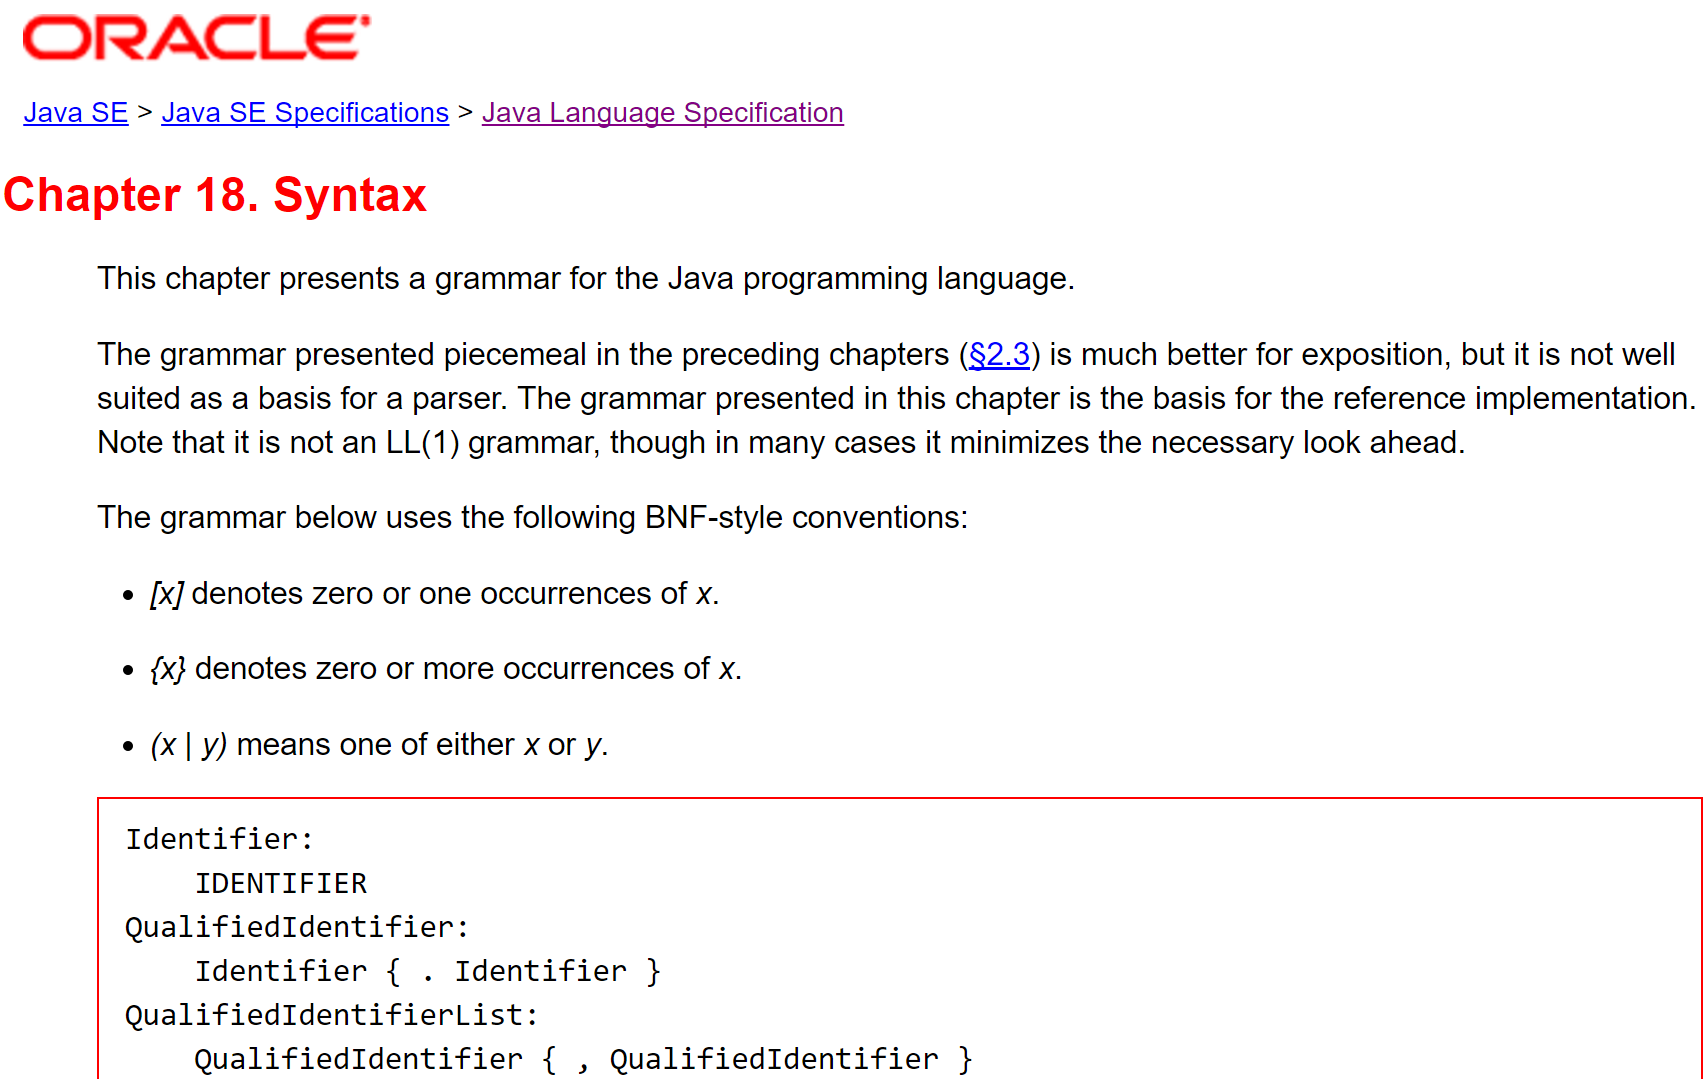
\includegraphics[width=12cm]{pictures/java_grammar.png}} 
%	\end{center}
%\end{frame}
\begin{frame}
     \frametitle{Биоинформатика}
     \begin{itemize}
         \item Множество задач, связанных с обработкой и пониманием биологических данных
         
         \item Геном --- длинная последовательность нуклеотидов
         \item На деле строка над алфавитом \{A, C, G, T\}
     \end{itemize}
 \end{frame}
 
 \begin{frame}
     \frametitle{Получение данных}
     \begin{tabular}{p{5cm} p{7cm}}
         \begin{itemize}
             \item Из биологического материала читаются короткие строчки
             \item Эти кусочки склеиваются в более длинные строки
             \item Множество строчек --- сборка
             \item Данных очень много, поэтому строится конечный автомат, пути в котором содержат полученные строки
         \end{itemize}
         &
         \begin{figure}[b]
             \centering
             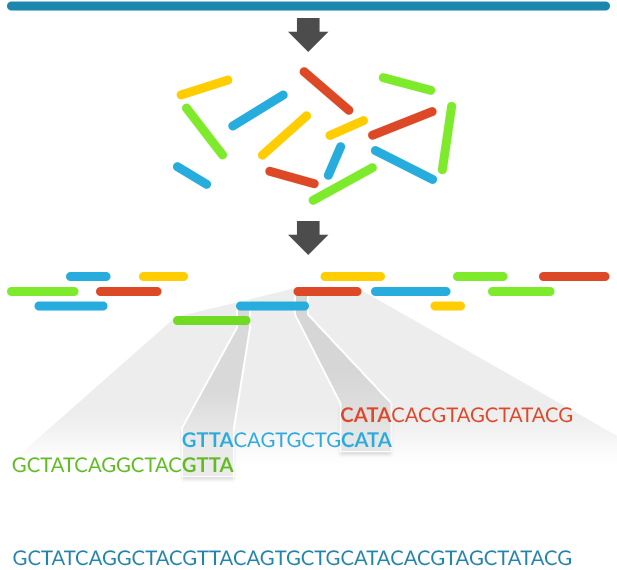
\includegraphics[width=6.5cm]{pictures/readsAssembly.png}  
         \end{figure}
     \end{tabular}
 \end{frame}
 
 \begin{frame}
     \frametitle{Метагеномная сборка}
     \begin{itemize}
         \item В сборке геномы различных организмов
         \item Нужно уметь определять содержащиеся в сборке огранизмы
     \end{itemize}
 \end{frame}
 
 \begin{frame}
     \frametitle{Как ищем}
     \begin{tabular}{p{6cm} p{5cm}}
         \begin{itemize}
             \item Такие последовательности как тРНК, 16s-рРНК позволяют провести классификацию организма
             \item Данные последовательности имеют общую вторичную структуру, которая может быть описана КС-грамматикой
         \end{itemize}
         &
         \vspace{-1cm}
         \begin{figure}[b]
             \centering
             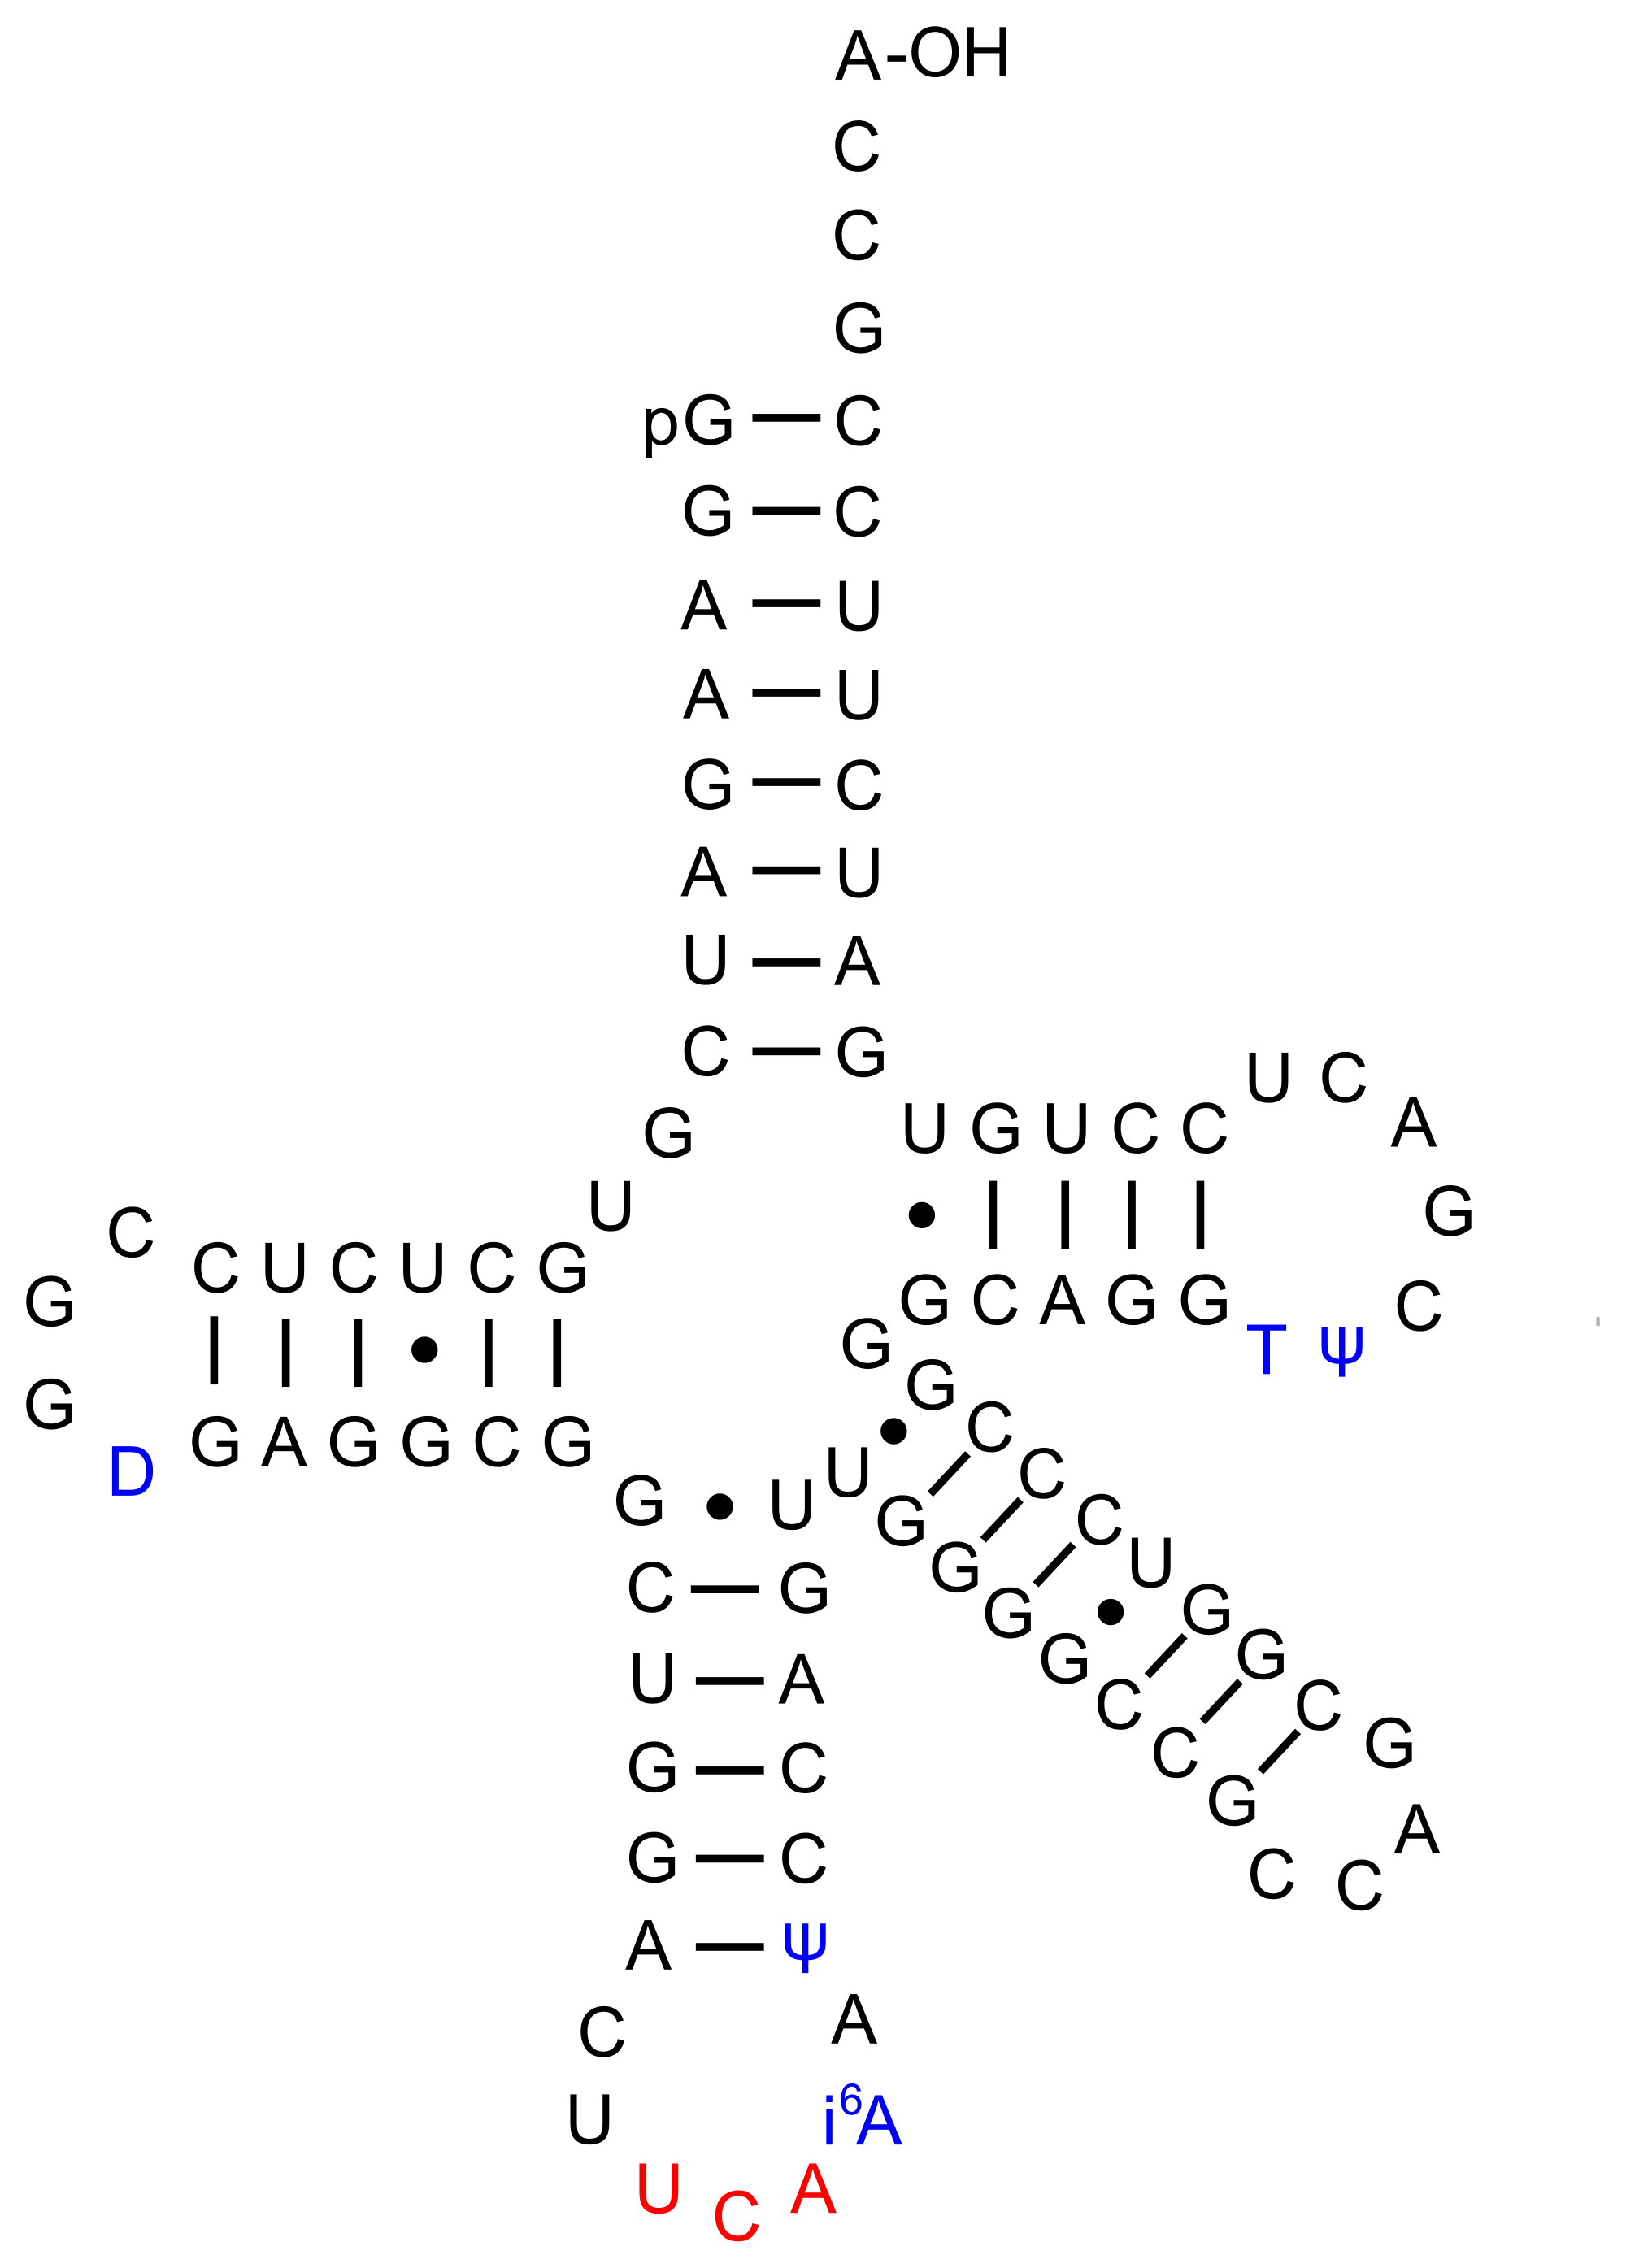
\includegraphics[width=5.2cm]{pictures/TRNA.png}
             \caption{Cтруктура тРНК}
         \end{figure}
     \end{tabular}  
 \end{frame}
 
 \begin{frame}
     \frametitle{Существующее решение}
     \begin{itemize}
         \item В магистерской прошлого года реализован алгоритм синтаксического анализа регулярных множеств
         \begin{itemize}
            \item Основан на алгоритме Generalised LL
            \item Умеет решать задачу поиска цепочек в конечном автомате, удовлетворяющих КС-грамматике
            \item Реализован в рамках проекта кафедры системного программирования YaccConstructor
         \end{itemize}
         
     \end{itemize}
 \end{frame}
	\begin{frame} 
		\frametitle{Расширенные контекстно-свободные грамматики}
		\begin{center}
		В правых частях продукций регулярные выражения
		\end{center}
		\begin{center}
			{$\begin{aligned}
				S\ =&\ a\ M^* \\
				M\ =&\ a?\ (B\ K)^+ \\
				|&\ u\ B \\
				B\ =&\ c\ |\ \varepsilon
				\end{aligned}$}
		\end{center}
	\end{frame}
	
%	\begin{frame}
%		\frametitle{Результат преобразования в BNF}
%		\begin{tabular}{c c}
%		7 нетерминалов & 18 нетерминалов
%		\\
%		\multicolumn{2}{c}{
%		\begin{columns}
%			\begin{column}{6.1cm}
%				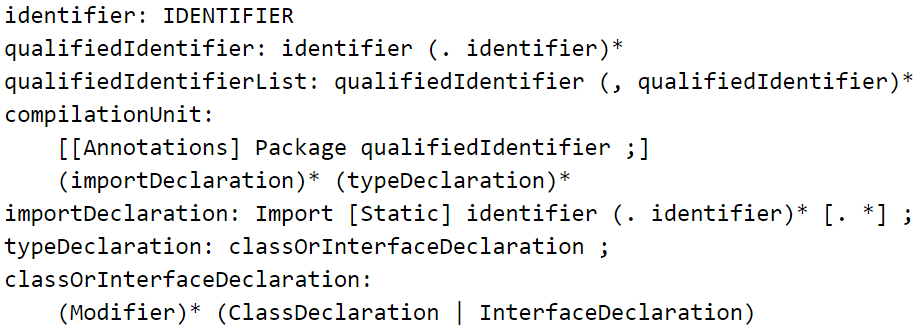
\includegraphics[width=6cm]{pictures/java_before.png}
%			\end{column}
%			\begin{column}{.7cm}
%				$ \Longrightarrow $
%			\end{column}
%			\begin{column}{5cm}
%				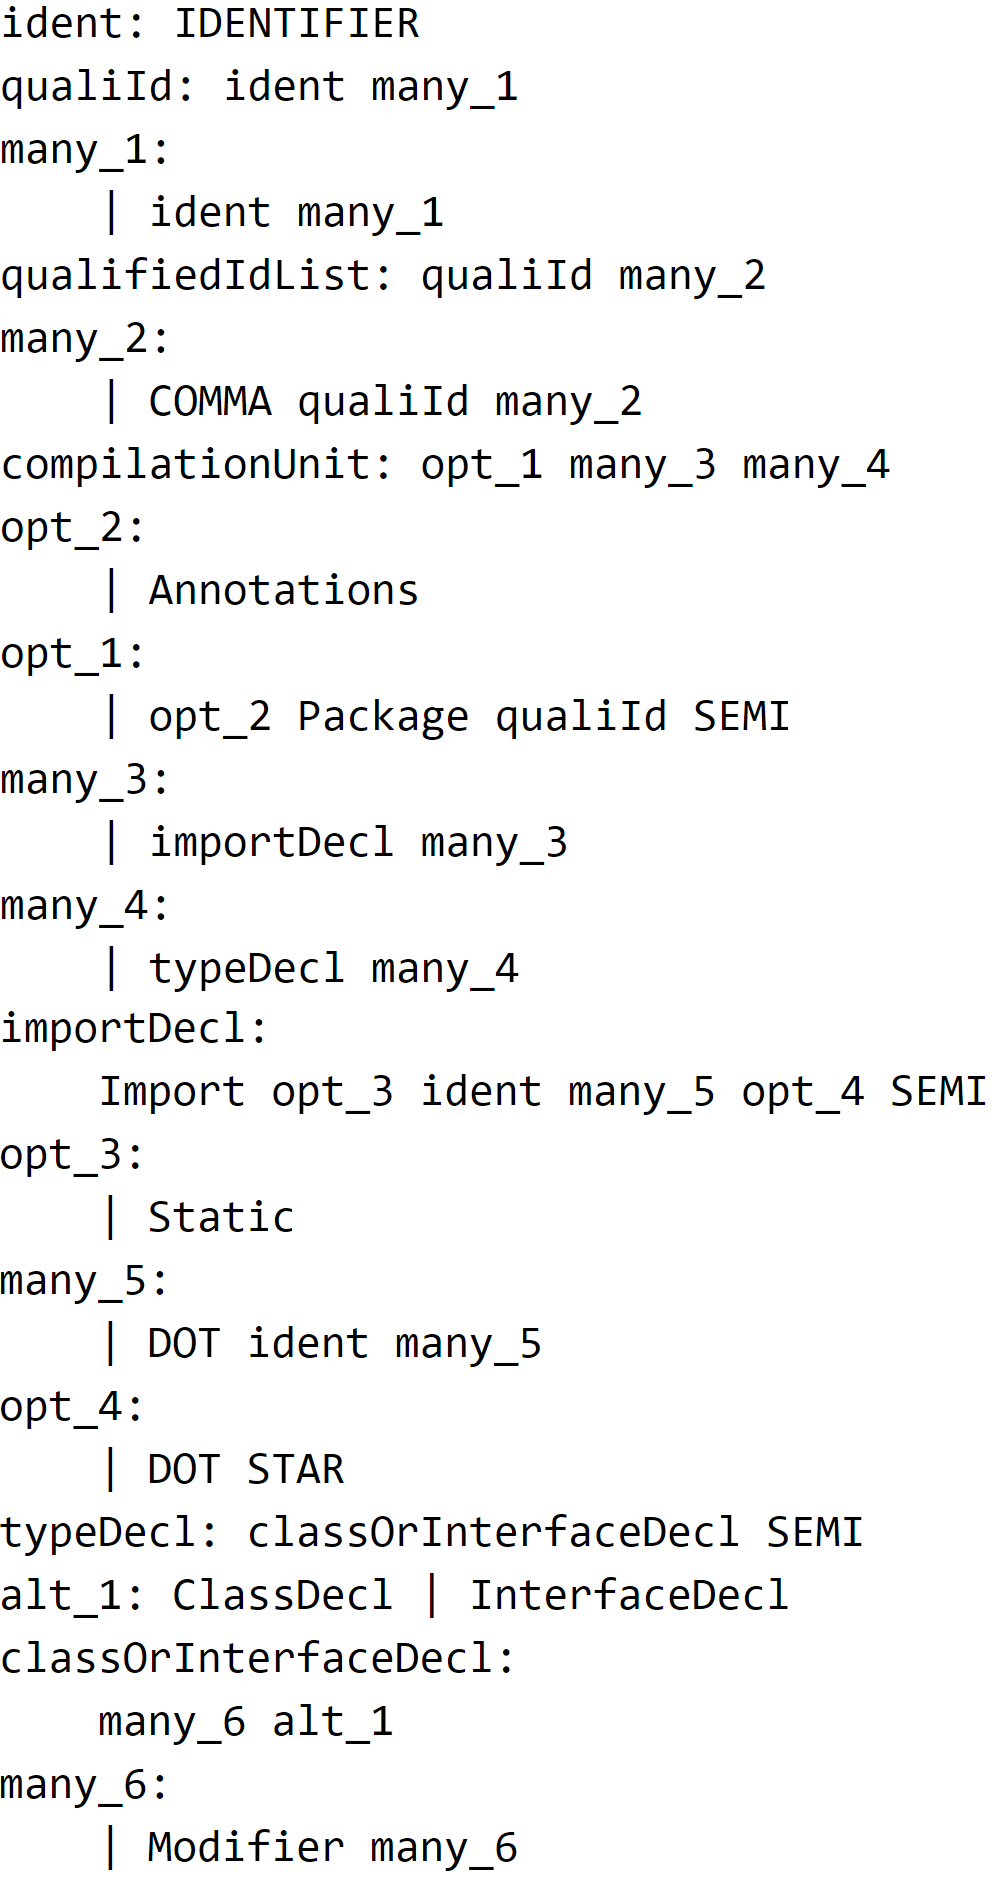
\includegraphics[width=3.5cm]{pictures/java_after.png}
%			\end{column}
%	    \end{columns}
%    }
 %       \end{tabular}
%	\end{frame}

%\begin{frame}
%	\begin{center} 
%		\only<1>{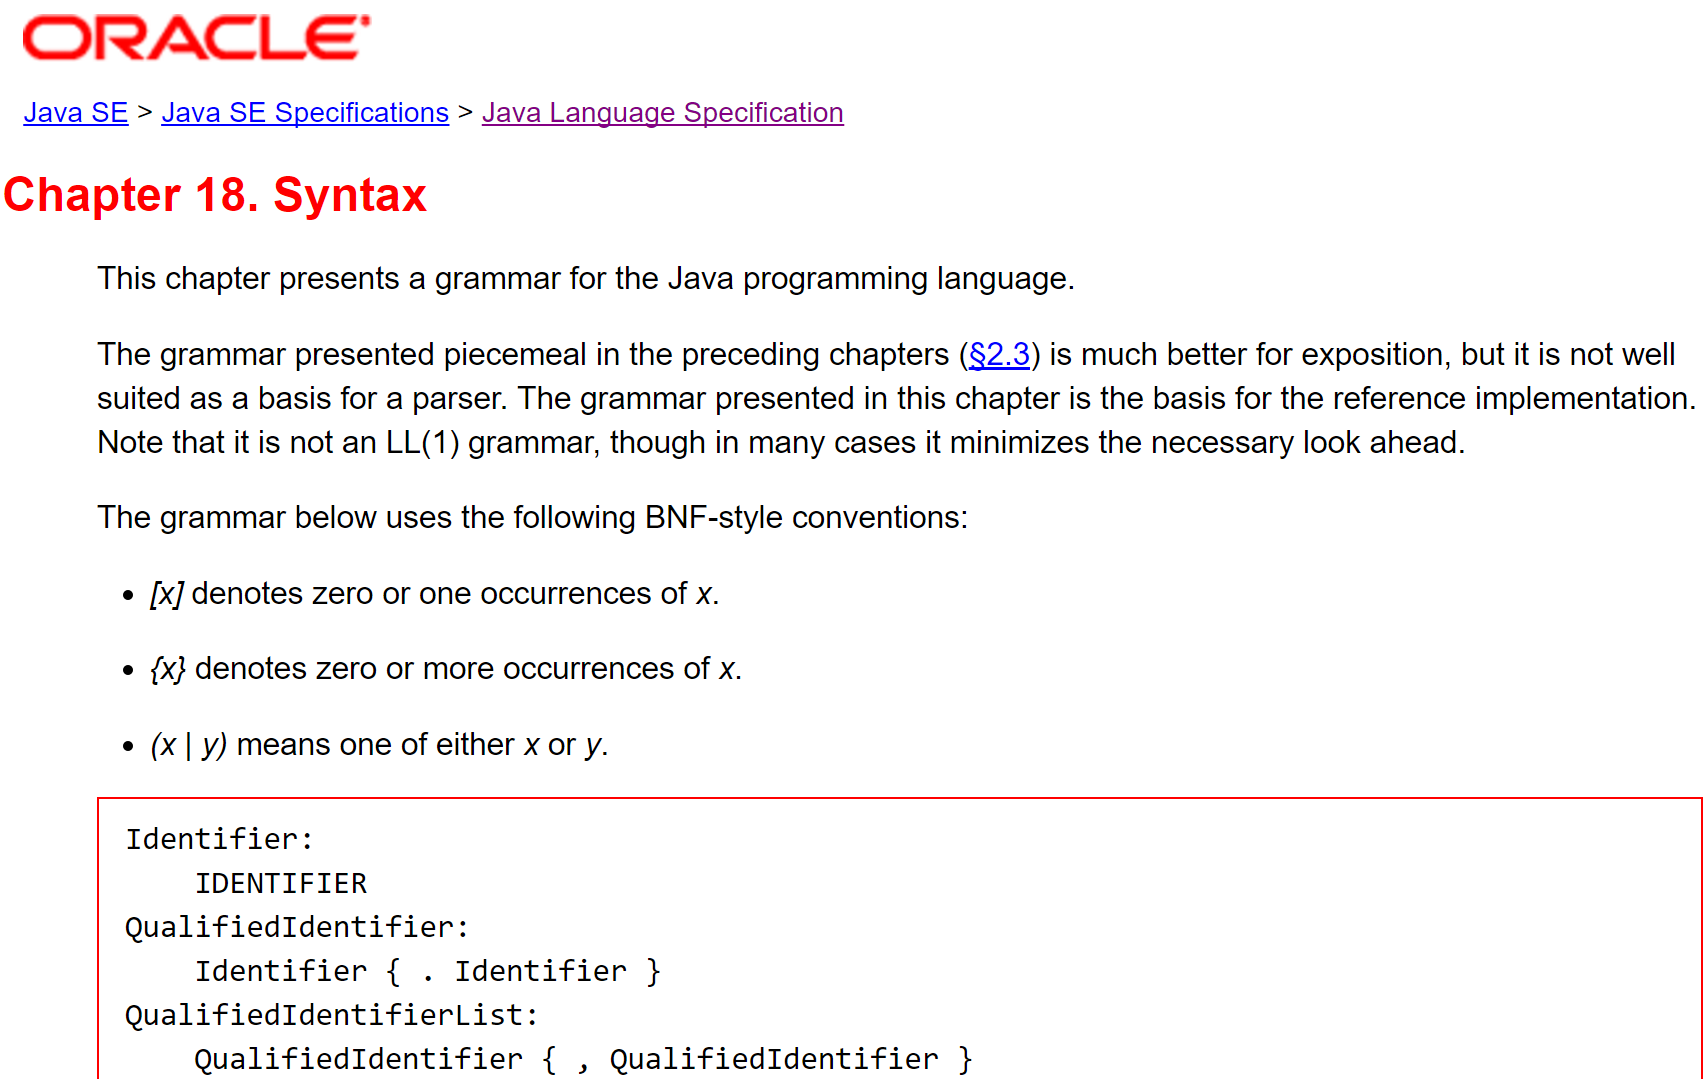
\includegraphics[width=12cm]{pictures/java_grammar.png}} 
%		\only<2>{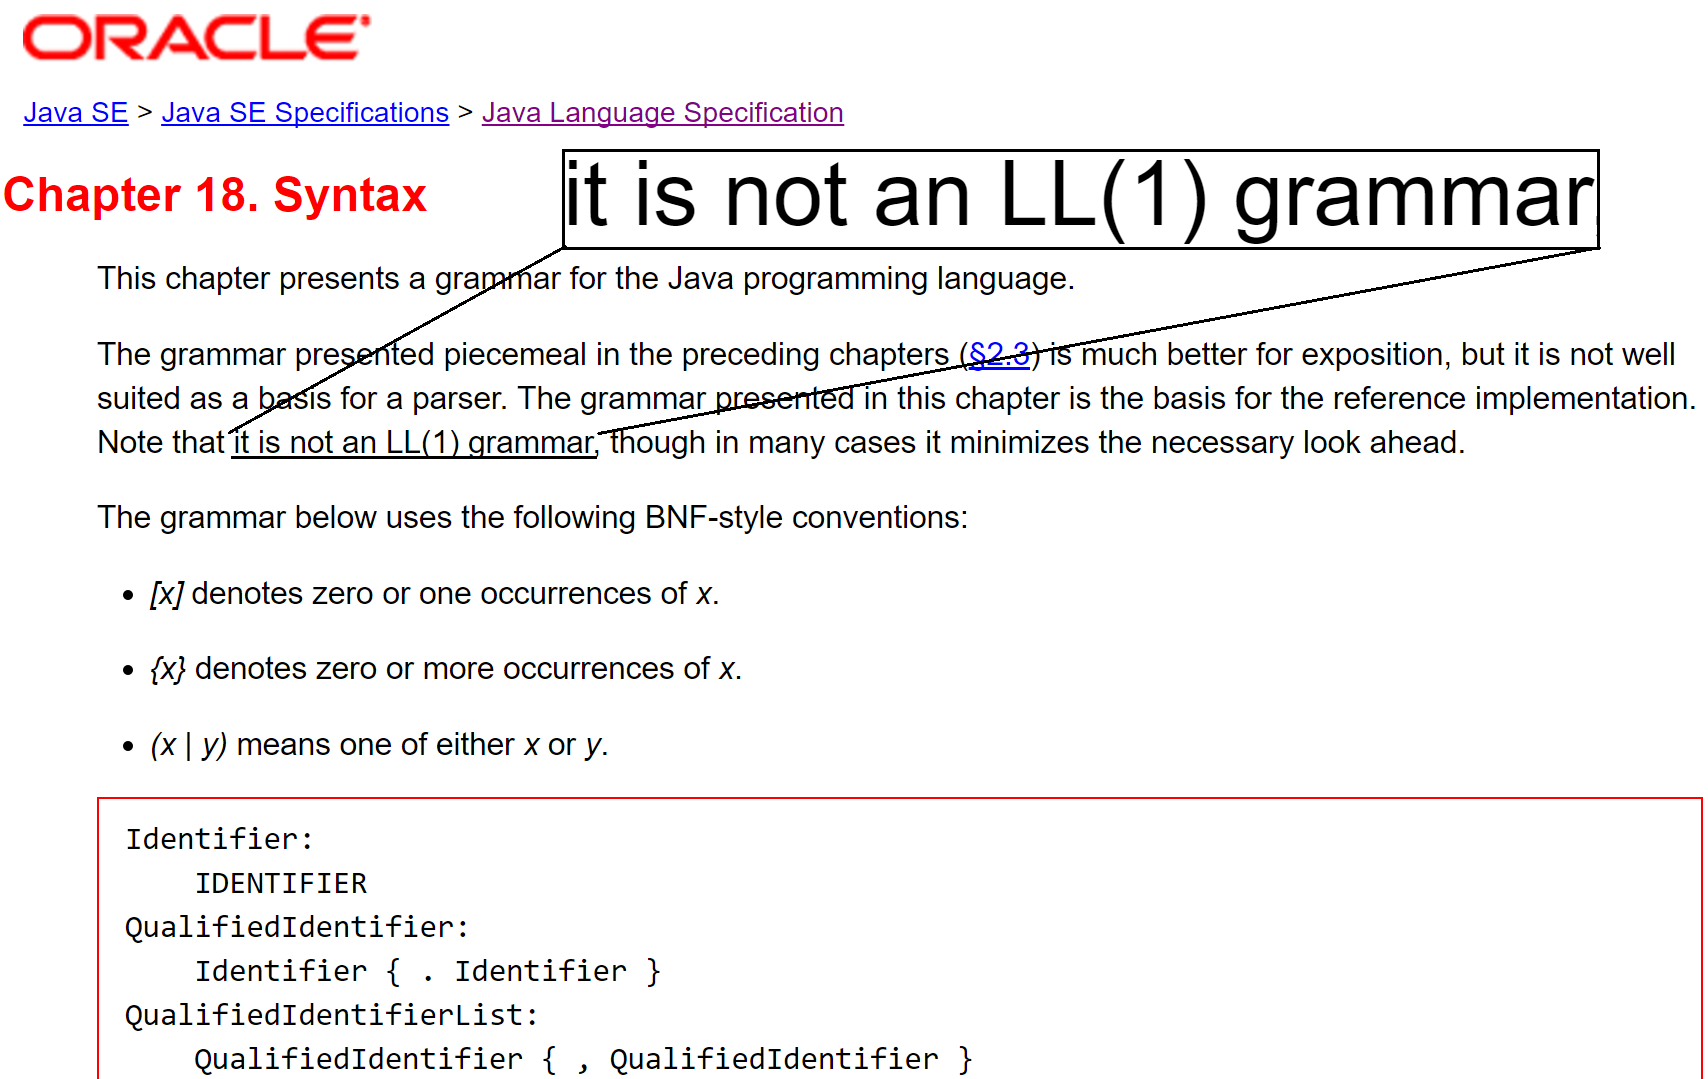
\includegraphics[width=12cm]{pictures/java_grammar_2.png}} 
%	\end{center}
%\end{frame}

	
	\begin{frame} 
		\frametitle{Обзор} 
		\begin{itemize}
			\item Теоретические работы о синтаксическом анализе ECFG
			\begin{itemize}
				\item L. Breveglieri, S. Crespi Reghizzi, A. Morzenti (2014). ELR parsing
				\item K. Hemerik.(2009) ECFG and RRPG Parsing
   			\end{itemize}
            \item Описываются лишь LL(k), LR(k) подходы
            \item Работать с LL проще чем с LR
        
            \item Нет инструментов допускающих произвольные ECFG
			\item \textbf{Generalised LL}
			\begin{itemize}
				\item Допускает произвольные CFG (включая неоднозначные)
				\item Не может использовать ECFG без преобразований
			\end{itemize}
		\end{itemize}
	\end{frame}

 

	\begin{frame} 
		\frametitle{Цель и задачи}
		Цель работы: разработать и реализовать модификацию алгоритма GLL, работающую с расширенными контекстно-свободными грамматиками, и проверить, как полученный алгоритм влияет на производительность поиска структур, заданных с помощью контекстно-свободной грамматики в метагеномных сборках.
		Для её достижения были поставлены следующие задачи:
		\begin{itemize}
			\item Выбрать или разработать подходящее представление ECFG
			\item Спроектировать структуру данных для представления леса разбора по ECFG
			\item Разработать алгоритм на основе Generalised LL, строящий лес разбора по ECFG
            \item Разработать механизм анализа регулярных множеств в алгоритме
			\item Реализовать алгоритм в рамках проекта YaccConstructor
			\item Провести экспериментальное сравнение реализованного алгоритма с существующим в проекте YaccConstructor при анализе метагеномной сборки
		\end{itemize}
	\end{frame}

	\begin{frame} 
		\frametitle{Автоматы и ECFG}
		
		\begin{columns}
			\begin{column}{4cm}
				Грамматика $G_0$\\
				\vspace{10pt}
				$
				\begin{array}[b]{rl}
				S = a^{*} S\ b? \ | \ c \ \ \ \ \ \ \ \ \  \Longrightarrow
				\end{array}
				$
			\end{column}
			\begin{column}{3.3cm}
				RA для грамматики $G_0$\\
				\vspace{10pt}
				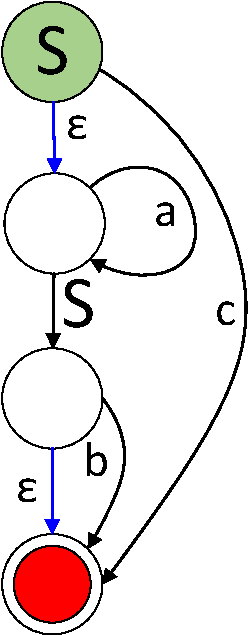
\includegraphics[width=2.5cm]{pictures/G0initialAutomaton.pdf}
			\end{column}
		\end{columns}
	\end{frame}

	\begin{frame} 
		\frametitle{Минимизация рекурсивных автоматов}
		\vspace{-12pt}
		\begin{center}
			%\begin{tabular}{c}
			{Грамматика $G_1$\\
			\vspace{5pt}
			$
			\begin{array}{rl}
			S =& K\ K\ K\ K\ K\ K \ |K\ a\ K\ K\ K\ K \\
			K =& S\ K\ |\ a\ K\ |\ a \\
			\end{array}
			$
			}
		    \\
		    \vspace{12pt}
		    Автомат для $G_1$
		    \\
		    \vspace{5pt}
		    {
				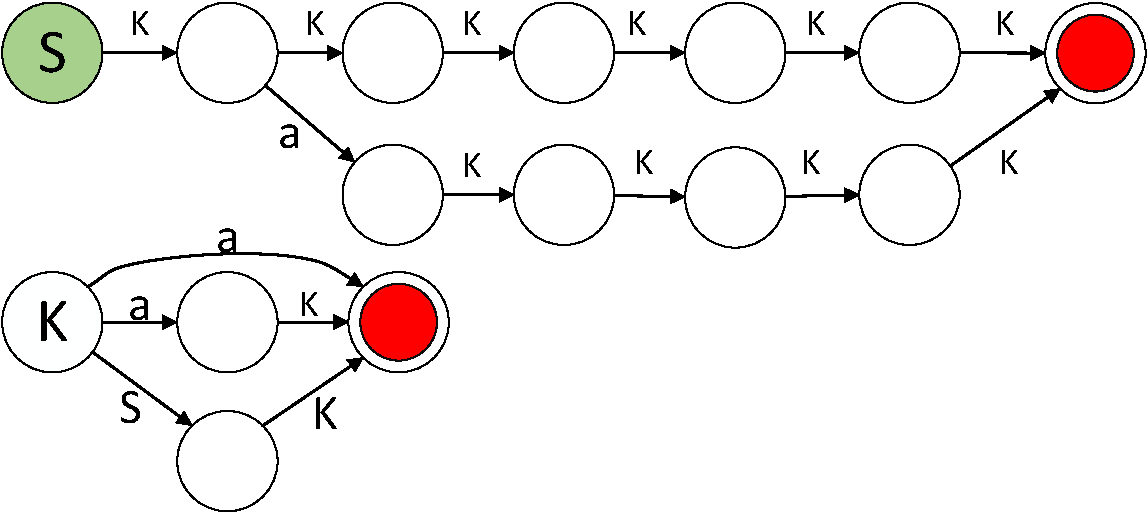
\includegraphics[width=7cm]{pictures/G1initial.pdf}
			}\\
			\vspace{8pt}
			Минимизированный автомат для $G_1$
			\\
			\vspace{5pt}
		    {
				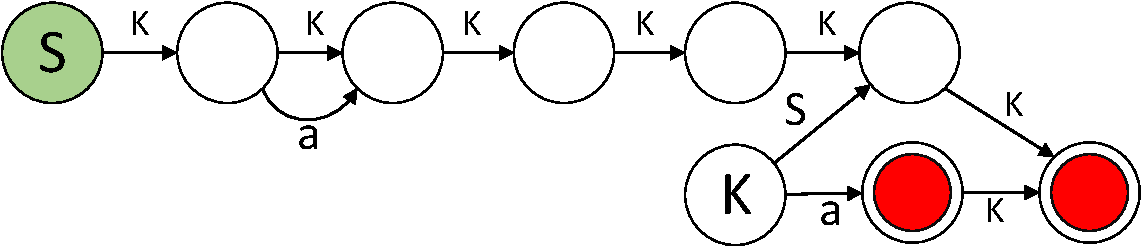
\includegraphics[width=7cm]{pictures/G1automaton.pdf}
			}
		\end{center}
	\end{frame}
	
	\begin{frame} 
		\frametitle{Деревья вывода для рекурсивных автоматов}
		%\vspace{-40pt}
		\begin{columns}
			\begin{column}{3.7cm}
				%Grammar: $$ S : a^{+} S\ b? \ | \ c $$
				Вход: $$aacb$$ \\
				\vspace{10pt}
				Автомат: \\
				\vspace{5pt}
				\begin{center}
					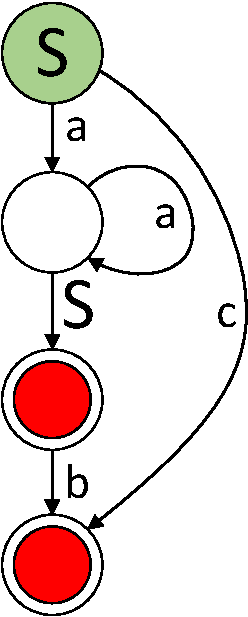
\includegraphics[width=2cm]{pictures/G0minimizedAutomaton.pdf}
				\end{center}
			\end{column}
		
     		\begin{column}{6cm}
     			\ \ Деревья вывода:\\
     			\vspace{5pt}
     			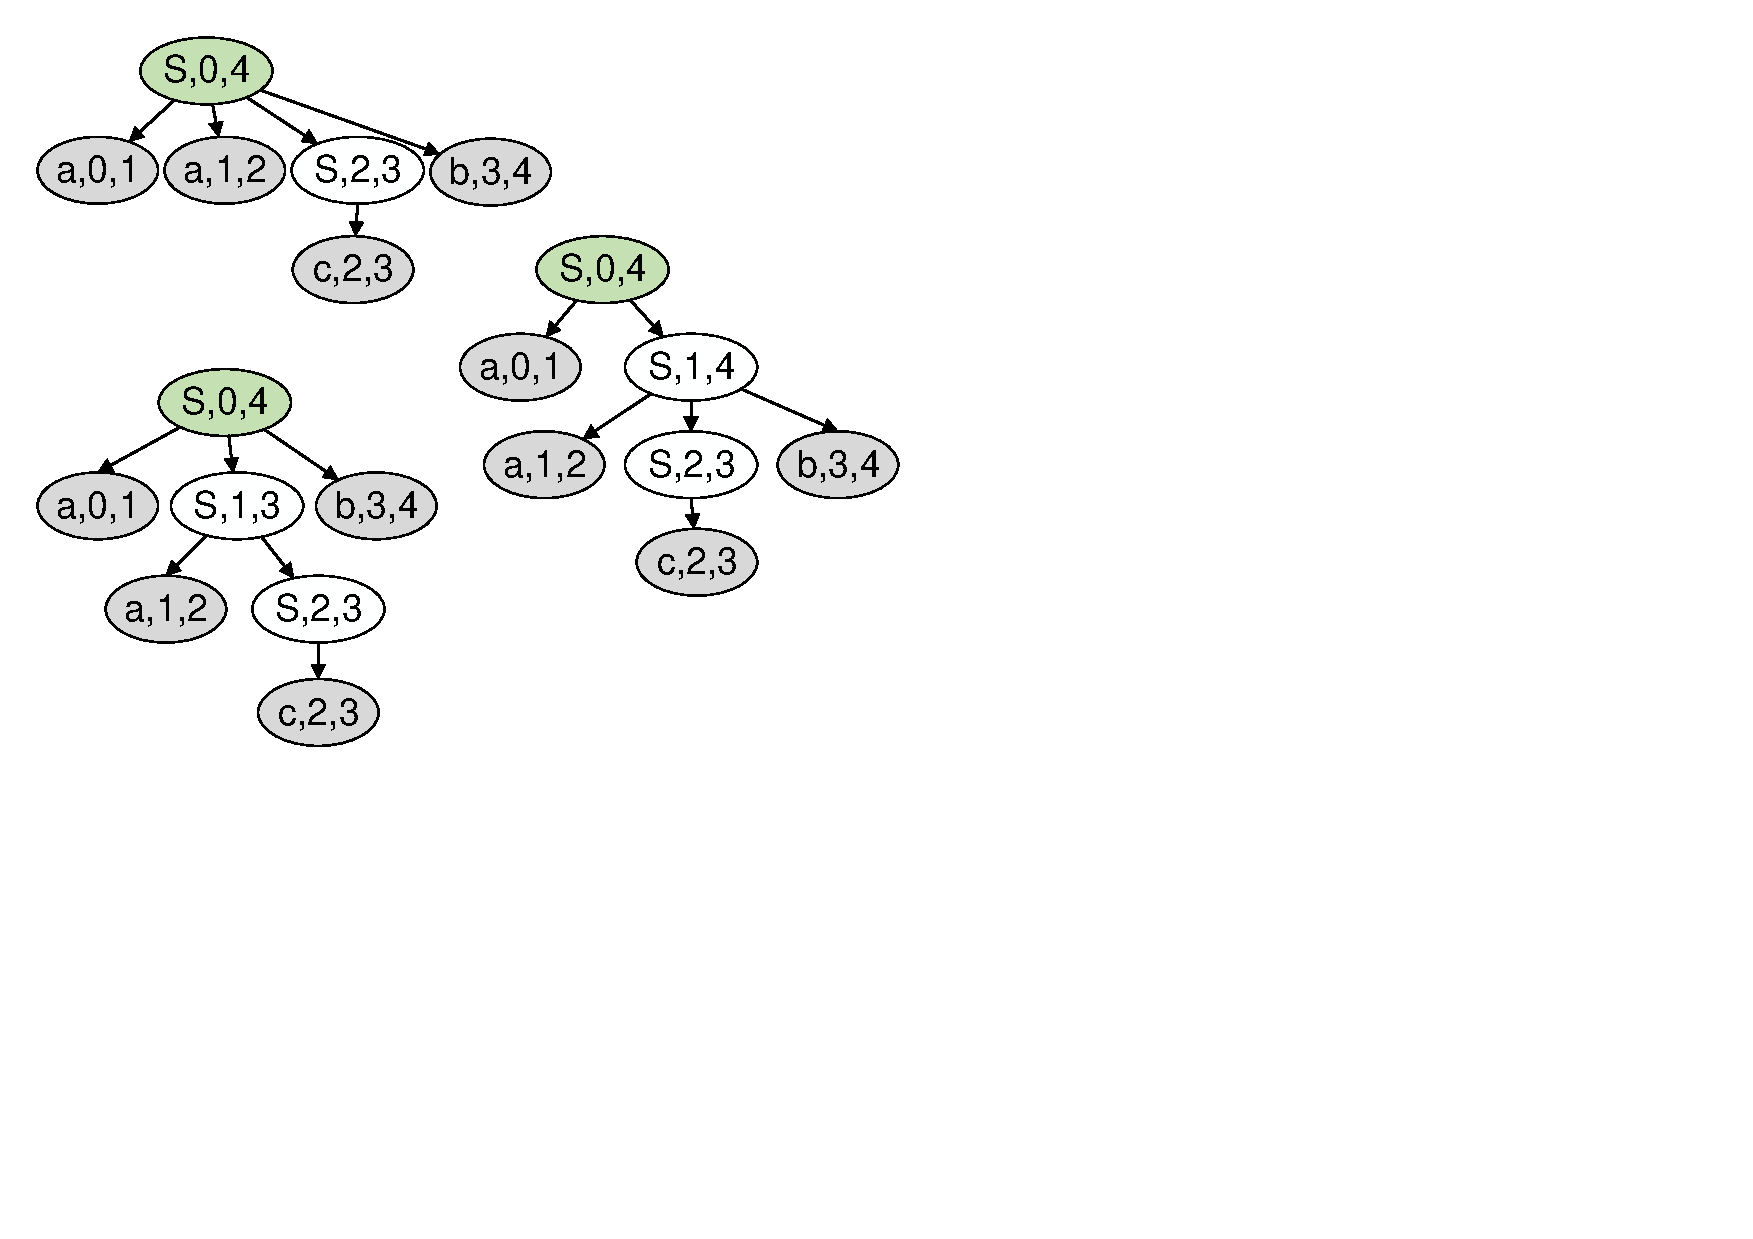
\includegraphics[width=7cm]{pictures/G0trees.pdf}
			\end{column}
		
		\end{columns}
	\end{frame}
	
	\begin{frame} 
		\frametitle{Разработанный алгоритм}
		\begin{itemize}
            \item Основан на Generalised LL
            \begin{itemize}
                \item Определено сжатое представление леса разбора(SPPF) для 
                рекурсивных автоматов
                \item Поддержаны рекурсивные автоматы вместо грамматик
            \end{itemize}
            \item Поддержан механизм анализа регулярных множеств
            \item Реализован в рамках проекта кафедры системного программирования YaccConstructor
		\end{itemize}
	\end{frame}
	
%	\begin{frame} 
%		\frametitle{Постоение леса разбора в оригинальном алгоритме}
%		\begin{itemize}
%			\item Очередь дескрипторов
%			\item Дескриптор (G, i, U, T) однозначно определяет состояние процесса разбора
%			\begin{itemize}
%				\item G - позиция в грамматике
%				\item i - позиция во входе
%				\item U - узел стека разбора
%				\item T - корень построенного леса разбора
%			\end{itemize}
%		\end{itemize}
%	\end{frame}
	%\begin{frame} 
%		\frametitle{Пример постоения леса разбора в оригинальном алгоритме}
%		\begin{columns}
%			\begin{column}{5cm}
%				Вход : \only<1-2>{$\ b c $}
%						\only<3-7>{$\bullet\ b c $} 
%						\only<8-11>{$b\bullet c $}
%						\only<12->{$b c \bullet$} \\
%				\vspace{15pt}
%				Грамматика: \\
%				\vspace{5pt}
%				\only<1>{$$
%					S = \ (a\ |\ b\ |\ S)\ c?
%					$$}
%				\only<2->{$
%				\begin{array}{rl}
%				S =&\only<3,6>{\bullet} \ a\ C\_opt \\
%				|&\only<4,7>{\bullet} \ b\only<8>{\bullet}\ C\_opt \\
%				|&\only<5>{\bullet} \ S\ C\_opt \\
%				C\_opt =& \only<9>{\bullet} \varepsilon \ | \only<10-11>{\bullet} \ c \only<12>{\ \bullet}\\
%				\end{array}
%				$}
%			\end{column}
%			
%			\begin{column}{5cm}
%				\only<3->{
%				\only<8>{\vspace{50pt}}
%				\only<12>{\vspace{44pt}}
%				\begin{center}Очередь дескрипторов\\\end{center}
%				\begin{tabu}{|[3pt]c|[3pt]}
%					\only<10>{$C\_opt =\bullet c$, 1, \dots, \dots \\ \hline}
%					\only<11->{\cellcolor{green!25}{$C\_opt =\bullet c$, 1, \dots, \dots} \\ \hline}
%					\only<11->{\st{$C\_opt =\bullet  \varepsilon$, 1, \dots, \dots} \\ \hline}
%					\only<9-10>{$C\_opt =\bullet  \varepsilon$, 1, \dots, \dots \\ \hline}
%					\only<5-10>{$S =\bullet \ S\ C\_opt$, 0, \dots, \dots \\ \hline}
%					\only<11->{\st{$S =\bullet \ S\ C\_opt$, 0, \dots, \dots} \\ \hline}
%					\only<3-4>{$\ \ \ \ \ \ \ \ \ \ \ \ \ \ \ \ \ \ \ \ \ \ \ \ \ \ \ \ \ \ \ \ \ \ $ \\}
%					%\strike{|[3pt]c|}{quux} & A & B \\
%					\only<4-6>{$S =\bullet \ b\ C\_opt$, 0, \dots, \dots \\ \hline}
%					\only<7-10>{\cellcolor{green!25}{$S =\bullet \ b\ C\_opt$, 0, \dots, \dots} \\ \hline}
%					\only<11->{\st{$S =\bullet \ b\ C\_opt$, 0, \dots, \dots} \\ \hline}
%					\only<3>{$\ \ \ \ \ \ \ \ \ \ \ \ \ \ \ \ \ \ \ \ \ \ \ \ \ \ \ \ \ \ \ \ \ \ $ \\}
%					\only<3-5>{$S =\bullet \ a\ C\_opt$, 0, \dots, \dots}
%					\only<6>{\cellcolor{green!25}{$S =\bullet \ a\ C\_opt$, 0, \dots, \dots}}
%					\only<7->{\st{$S =\bullet \ a\ C\_opt$, 0, \dots, \dots}}
%				\end{tabu}
%			}
		
%			\only<8>{
%				\vspace{20pt}
%				\begin{center}
%					\only<8>{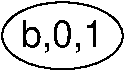
\includegraphics[width=2cm]{pictures/example_trees_b.pdf}}
%				\end{center}				
%			}
%			\only<12>{
%				\begin{center}
%					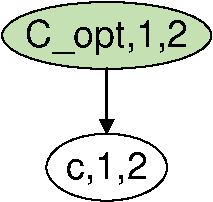
\includegraphics[width=2cm]{pictures/example_trees.pdf}
%				\end{center}				
%			}
%			\end{column}
%		    
%		\end{columns}
%	\end{frame}

%\begin{frame}
%	\frametitle{Постоение леса разбора по автомату}
%	\begin{itemize}
%		\item Очередь дескрипторов
%		\item Дескриптор (G, i, U, T) однозначно определяет состояние процесса разбора
%		\begin{itemize}
%			\item G - состояние автомата
%			\item i - позиция во входе
%			\item U - узел стека разбора
%			\item T - корень построенного леса разбора
%		\end{itemize}
%	\end{itemize}
%\end{frame}

%	\begin{frame} 
%		\frametitle{Пример постоения леса разбора по автомату}
%		\begin{columns}
%			\begin{column}{5cm}
%				Вход : $\only<1>{\ \ }\only<2->{\bullet} \ b c $ \\
%				\vspace{15pt}
%				Автомат : \\
%				\vspace{5pt}
%				\only<1>{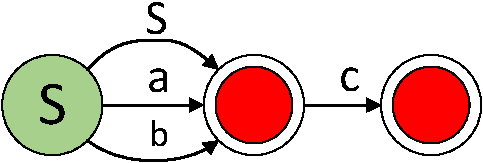
\includegraphics[width=5cm]{pictures/G2.pdf}}
%				\only<2>{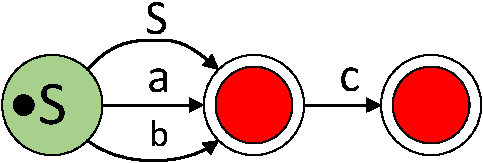
\includegraphics[width=5cm]{pictures/G2_1.pdf}}
%				\only<3>{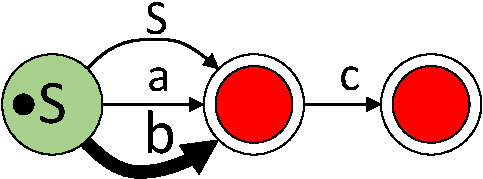
\includegraphics[width=5cm]{pictures/G2_2.pdf}}
%			\end{column}
%			\begin{column}{3cm}
%				%\only<3>{\vspace{50pt}}
%				\begin{center}
%				\only<2>{
%				Очередь дескрипторов\\
%				\begin{tabu}{|[3pt]c|[3pt]}
%					\only<2->{$S$, 0, \dots, \dots}
%				\end{tabu}
%				}
%				\only<3>{
%					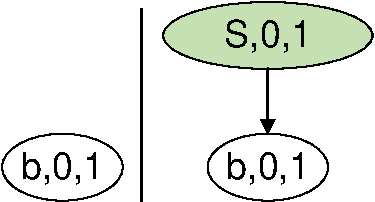
\includegraphics[width=4cm]{pictures/example_trees_auto.pdf}
%				}
%				\end{center}
%			\end{column}
%		\end{columns}
%	\end{frame}

%\begin{frame}
%	\frametitle{Реализация}
%	Алгоритм реализован в рамках проекта YaccConstructor
%	\begin{itemize}
%		\item Архитектура проекта модульная, поэтому понадобилось лишь встроить непосредственно генератор парсеров
%		\item .net, $F\#$
%	\end{itemize}
%\end{frame}

\newcolumntype{C}[1]{>{\centering\let\newline\\\arraybackslash\hspace{0pt}}m{#1}}
	
	\begin{frame} 
		\frametitle{Эксперименты}
		\begin{center}
            \begin{columns}
        	    \begin{column}{4.1cm}
          	     Грамматика $G_1$
                   \vspace{2pt}
                $
                \begin{array}{rl}
                S =& K(\ K\ K\ K\ K\ K \ \\
                &| a\ K\ K\ K\ K) \\
                K =& S\ K\ |\ a\ K\ |\ a \\
                \end{array}
                $
       			\end{column}
       			\begin{column}{6cm}
            				Результаты для входа $a^{450}$
                \\
                \vspace{2pt}
                \begin{tabular}{ | c | c | c | }
                    \hline
                    %& \rotatebox[origin=c]{90}{Время}
                    %& \rotatebox[origin=c]{90}{Дескрипторы} &
                    %\rotatebox[origin=c]{90}{Рёбра GSS} &
                    %\rotatebox[origin=c]{90}{Узлы SPPF} &
                    %\rotatebox[origin=c]{90}{Память, Мб} \\ \hline
                    & Время &   Память,Мб\\ \hline
                    Гамматика& 10мин.13с.  &  11818 \\ \hline 
                    RA       & 5мин.51с.  & 8026  \\ \hline \hline
                    Ratio   &  43$\%$       &  33 $\%$ \\ \hline
                \end{tabular}
            			\end{column}
	    \end{columns}
		%\\
		%\vspace{5pt}
		%Рекурсивный автомат для грамматики $G_1$
		%\\
		%\vspace{3pt}
		%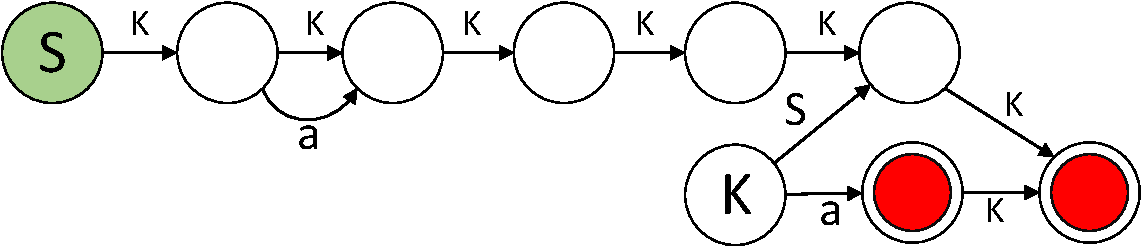
\includegraphics[scale=.5]{pictures/G1automaton.pdf}
		%\\
		%\vspace{5pt}
    \begin{tikzpicture}[scale=.7]
    \begin{axis}[
    legend cell align=left,
    legend pos = north west,
    xlabel = {Длина входа},
    ylabel = {Память, Мб},
    %ymode=log
    ]
    \addplot [only marks, mark=triangle*] coordinates {
        (90,130) (120,267) (150,491) (180,842) (210,1318) (240,1977) (270,2827) (300,3869) (330,5183) (360,6665) (390,8583) (420,10671) (450,11818)
    };
    \addplot [only marks, mark=*] coordinates {
        (90,106) (120,190) (150,325) (180,531) (210,829) (240,1225) (270,1728) (300,2359) (330,3161) (360,4126) (390,5242) (420,6571) (450,8026)
    };
    \legend{ 
        Грамматика, 
        Автомат
    };
    \end{axis}
    \end{tikzpicture}
    \begin{tikzpicture}[scale=.7]
    \begin{axis}[
    legend cell align=left,
    legend pos = north west,
    xlabel = {Длина входа},
    ylabel = {Время, с},
    %ymode=log
    ]
    \addplot [only marks, mark=triangle*] coordinates {
        (30,00.1690245) (60,01.1310924) (90,03.6899218) (120,11.1006359) (150,20.8163584) (180,28.7973458) (210,45.3640866) (240,68.3269546) (270,102.2953852) (300,150.2681210) (330,197.9508999) (360,269.1387530) (390,346.4999998) (420,442.0947044) (450,613.3386222)
    };
    \addplot [only marks, mark=*] coordinates {
        (30,00.0625041) (60,00.6562026) (90,02.6719009) (120,04.3594156) (150,09.2969549) (180,15.6406979) (210,25.3438039) (240,39.1251338) (270,57.6720586) (300,82.0470354) (330,109.7031754) (360,150.5466896) (390,191.5317906) (420,241.1571067) (450,351.8283519)
    };
    \legend{ 
        Грамматика, 
        Автомат
    };
    \end{axis}
    \end{tikzpicture}
        \end{center}
		%\begin{tabular}{ | c | c | c | c | c | }
		%	\hline
		%	\multirow{2}{*}[-1ex]{} &\multicolumn{3}{c|}{Использование памяти} & \multirow{2}{*}[-1ex]{Время, с} \\
		%	\cline{2-4}
        %     &  Дескрипторы & Рёбра стека & узлы SPPF &    \\ \hline
		%	Грамматика &  7,940        & 6,974      & 111,127,244 & 81 \\ \hline
		%     RA &  5,830        & 4,234      & 74,292,078  & 54 \\ \hline \hline
		%	Ratio   &  27$\%$       & 39$\%$     & 33 $\%$ & 35 $\%$    \\ \hline
		%\end{tabular}
		%\end{center}
	\end{frame}

	\begin{frame} 
		\frametitle{Поиск в метагеномных сборках} 
        \begin{itemize}
            \item Были проведены эксперименты на метагеномной сборке
            \item 10 компонент с 400-100 состояний и переходов и 1118 компонент с менее чем 100 состояний и переходов
        \end{itemize}
		\begin{center}
            
		\vspace{40pt}
		\begin{tabular}{ | c | c | c | }
			\hline
			             &  Память & Время   \\ \hline
			Существующее решение  &  27 Гб   & 02.26 мин \\ \hline
			Предложенное в данной работе &  10  Гб   &  01.25 мин \\ \hline \hline
			Ratio   &  63 $\%$     &  45 $\%$ \\ \hline
		\end{tabular}
		\end{center}
	\end{frame}

	\begin{frame} 
		\frametitle{Результаты}
		\begin{itemize}
			\item В качестве подходящего представления ECFG предложены рекурсивные автоматы
			\item Определён SPPF для ECFG
			\item Разработан алгоритм на основе GLL, строящий SPPF по ECFG
            \item Разработан механизм анализа регулярных множеств в алгоритме
			\item Алгоритм реализован в рамках проекта YaccConstructor
			\item Эксперименты показали двухкратный прирост производительности по сравнению с существующим решением 
			\item Выступление на международной конференции ``Tools and Methods of Program Analysis''(Москва, 2017г.)
		\end{itemize}		
	\end{frame}
\end{document}